Clustering is the process of organizing a set of objects into groups in which the objects within each group are more similar to each other than to those in other groups. In the study of complex networks, it is claimed that a network has a community structure if the nodes of the network can be easily divided into groups with a high level of internal connections. See an example of a network with community structure in Figure \ref{fig:example_communities}.

\begin{figure}[!htb]
    \centering
    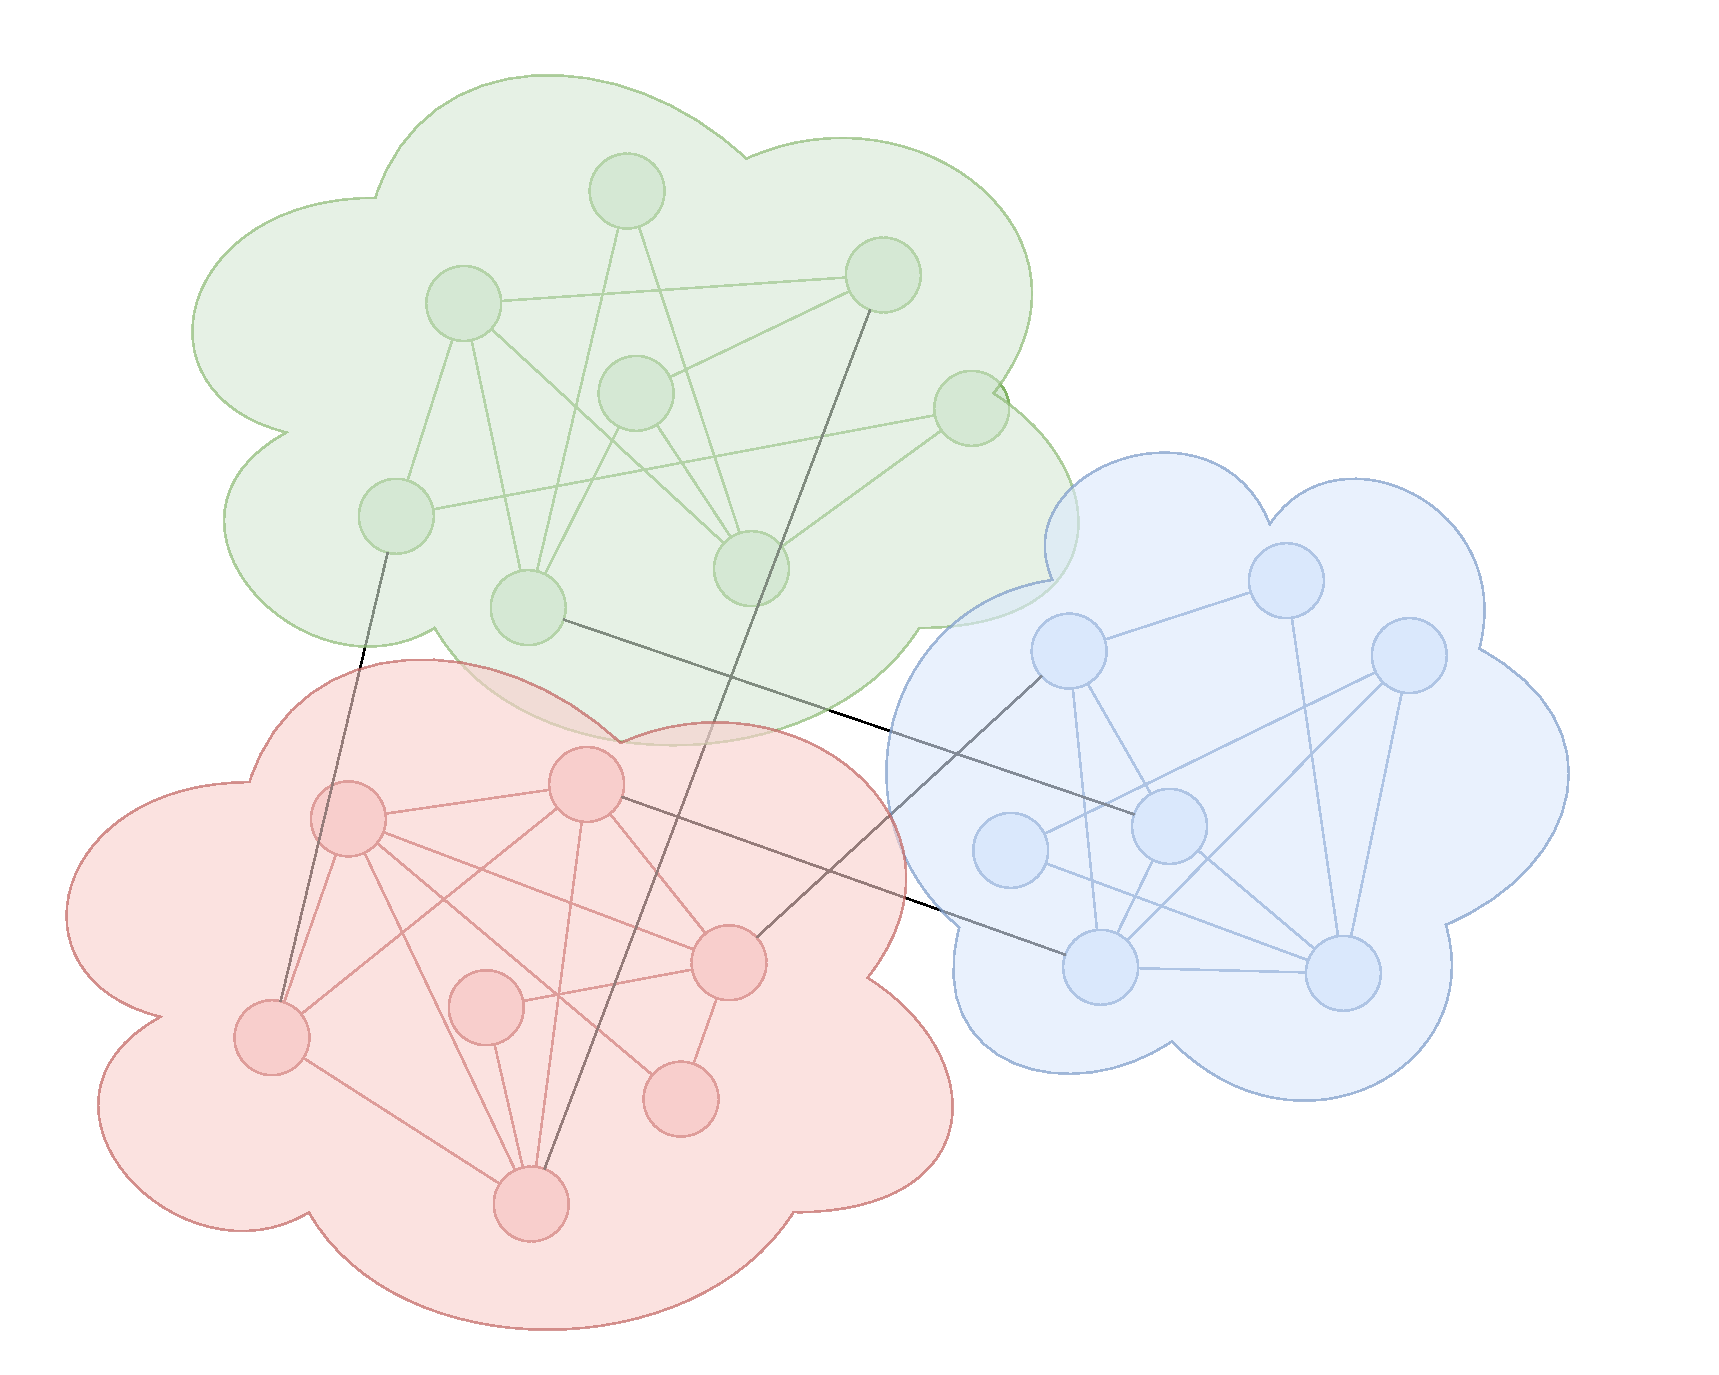
\includegraphics[width=0.6\textwidth]{images/network_w_community.pdf}
    \caption{A schematic representation of a network with community structure. In this network there are three communities of densely connected vertices with a much lower density of connections between them. Extracted and adapted from \cite{doi:10.1073/pnas.122653799}.}
    \label{fig:example_communities}
\end{figure}

Discovering a community structure in a real network is a frequent occurrence. It is essential to identify any existing underlying community structure in a network for a variety of reasons. For example, in a protein interaction network, communities are associated with proteins that have similar functions within a biological cell \cite{Zare2010}. Similarly, the presence of communities can have an impact on a wide range of behaviors, including the propagation of rumors and the transmission of epidemics in a network \cite{UCAM-CL-TR-767, ReisPinheiro2021}.

We have observed that the identification of communities is of great importance in various fields. The report will examine different community detection algorithms in terms of a variety of metrics. We will assess the performance of our methods by utilizing a set of 4 networks, ranging from real-world networks to artificial ones, some of which have known ground-truth communities and some with unknown communities.

This document is divided into four different sections. Next, our results are presented in Section \ref{sec:results}. Discussion and conclusions are covered in section \ref{sec:discussion}, and finally, some aspects of the methodology are presented in section \ref{sec:methods}.
